\documentclass{article}


% *** *** *** %
\usepackage{indentfirst}
\usepackage{graphicx}
\usepackage{url}
\usepackage{tikz}
\usepackage{subfigure}
\usepackage{microtype}
\def\tm{\leavevmode\hbox{$\rm {}^{TM}$}} %\tm
\newcommand{\cs}{C\slash S}
% *** *** *** %


\begin{document}

\title{Egal Car: A Synchronized Peer-to-Peer Car Racing Game Over Named Data Networking}
\author{Zening Qu}
\date{\today}
\maketitle

\begin{abstract}
Blahblahblah
\end{abstract}

%============================================================================%
\section{Introduction}
\label{introduction}

One of the most important differences between a multiplayer on-line game (MOG) and a single player game is that in the former case there exists a virtual world that needs to be shared and maintained \emph{consistent}. Consistency maintenance is about guaranteeing that all players in the shared virtual world will have correct understanding of it. For example, in a game that provides a global view to its players, everyone should be able to view the position of all other players in real time, and there should not be any collision between any two views. 

Synchronization mechanisms are fundamental to consistency maintenance. In a MOG where players are usually distributed in a wide geographic area, delivery of game state updates relies solely on the packets transmitted through the network. If the lower layers only provide connectionless services, which is highly possible since MOGs typically use IP and UDP, it can be imagined that those packet updates will be out of order when received by players. This is a potential hazard to MOGs because normally game state updates should be processed in the order of their generation time in order for players to learn the chronological and causal relationship between updates. If packets were not processed in the correct order, different players would have different understanding of the game state. In other words, \emph{inconsistency} would arise. A synchronization mechanism avoids inconsistency by making sure that all players process update packets in the correct order (see section~\ref{ndnbackground}). With a synchronization mechanism every copy of the game application receives consistent input from the network, therefore their outputs will be consistent, too.
\footnote{Note that game state consistency can also be achieved by using connection-oriented protocols such as TCP in the lower layers. However, research has shown that such protocols may result in severe performance degradation and thus are rarely used by MOGs~\cite{Fgame}.}

This paper documents a simple synchronization mechanism that we designed for MOGs over named data network (NDN)~\cite{Jndn}. NDN is a new Internet architecture that names data instead of hosts (see section~\ref{ndnbackground}). From the game application's point of view, NDN can be regarded as a new lower layer service provider, or an alternative of TCP\slash IP. But NDN's impact on game development and synchronization mechanism may go beyond that: as data acquire names that are meaningful to game applications, the method for managing and synchronizing these data evolves accordingly. % :)

We explored NDN's impact on MOG design and implementation by creating a MOG on our NDN testbed. Our game prototype is called \emph{Egal Car}, which is a 3D car racing game with highly detailed scenery and track. Each player has control over one car, which can speed up, slow down and alter direction. The cars can collide with each other and with fences along the track. All car movements are simulated by the game's physics engine. Like in any racing game, each player's goal is to lead the other competitors and win the race. Note that Egal Car is adapted from an open source game template called Unity\tm  Car Tutorial~\cite{UnityCar}. This template provides all graphics and physics modules that we mentioned above, but does not contain a network module. In other words, the template is a single-player off-line car racing game with all front-end work done; it only takes a network module to become a MOG. We designed and engineered the network module of this game. Specifically, we designed a synchronization mechanism with the car racing game's needs in mind. 

The rest of this paper describes the design choices and implementation details of our prototype game and its network module. Section~\ref{ndnbackground}~introduces NDN principles and facts that may inspire MOG design. Sections~\ref{architecture}~through~\ref{implementation}~discuss MOG design, using Egal Car as a main example.


%============================================================================%
\section{NDN Background}
\label{ndnbackground}

NDN differs from IP in that every piece of NDN data can have a \emph{name} that is meaningful to its consumer (the application who processes the data). To retrieve a piece of data, the receiver must know the data's name, but he/she does not have to know the data's location (host address) as in the IP network. NDN communication is established on the two packet types: \emph{Interest} and \emph{Data}. An Interest is a packet issued by the data receiver to express that a certain piece of data is needed. A Data is a packet published by the sender in response to an Interest. Both Interest and Data use names to identify the data being exchanged (see figure~\ref{img:packet_types}). An Interest is `satisfied' by a Data if its Content Name is a prefix of the Content Name in the Data packet.~\cite{Jndn}

\begin{figure}
\begin{center}
\includegraphics[width=0.7\textwidth] {image/packet_types}
\caption{Interest packet and Data packet}
\label{img:packet_types}
\end{center}
\end{figure}

% introduce CCNx and Sync
There are a few general purpose synchronization protocols under development. Among them is the CCNx Synchronization Protocol~\cite{CCNxSync} (CCNx Sync). CCNx\textregistered~is an implementation of NDN and open source project of PARC\textregistered. CCNx Sync is a facility provided by the CCNx project to help applications to maintain data integrity. It should be noted that, CCNx Sync, and other general purpose synchronization protocols are different from the game synchronization mechanisms that we mentioned in section~\ref{introduction}. The general purpose protocols maintain data integrity while the game protocols ensure game state consistency. Nevertheless, CCNx Sync can be utilized by MOGs in many situations. In fact, through our experiment we found that CCNx Sync brings lots of conveniences to MOG development. We demonstrate the use of CCNx Sync in Egal Car in section~\ref{synchronization}.


%============================================================================%
\section{Architecture}
\label{architecture}

When designing the network module of a MOG, the first decision that should be made is what architecture the MOG should use. Game architecture is a defining factor of the game's scalability, robustness and performance, and it has a fundamental influence on other game design choices such as the choice of synchronization mechanisms. As the network transmission strategy has changed in NDN, the preference of game architectures may also change.

There are two classes of game architectures, Client\slash Server (\cs) and Peer-to-Peer (P2P). In \cs~architectures all clients are directly connected to a central server which is the only authorized source of game state updates (see figure~\ref{cs}). In P2P architectures, peers (clients) are inter-connected and each peer computes newer game state on its own (see figure~\ref{p2p}). 

\begin{figure} 
\centering  
\subfigure[\cs]  
{  
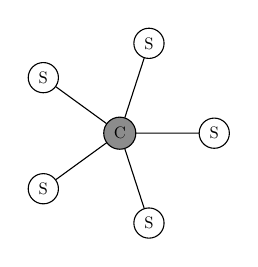
\begin{tikzpicture} [scale=0.6, transform shape]
\tikzstyle{every node}=[draw,shape=circle];
\node [fill = gray!90] (v0) at (0:0) {C};
\node (v1) at ( 0:2) {S};
\node (v2) at ( 72:2) {S};
\node (v3) at (2*72:2) {S};
\node (v4) at (3*72:2) {S};
\node (v5) at (4*72:2) {S};
\draw (v0) -- (v1) % star
(v0) -- (v2)
(v0) -- (v3)
(v0) -- (v4)
(v0) -- (v5);
\end{tikzpicture}
\label{cs}
}  
\subfigure[P2P]  
{  
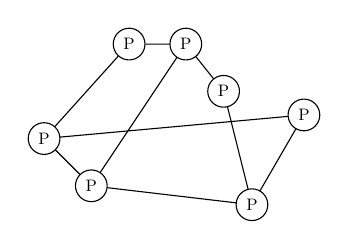
\begin{tikzpicture} [scale=0.6, transform shape]
\tikzstyle{every node}=[draw,shape=circle];
\node (v0) at (0, 2) {P};
\node (v1) at (1, 1) {P};
\node (v2) at (1.8, 4) {P};
\node (v3) at (3, 4) {P};
\node (v4) at (4.4, 0.6) {P};
\node (v5) at (3.8, 3) {P};
\node (v6) at (5.5, 2.5) {P};
\draw (v0) -- (v1)
(v0) -- (v2)
(v0) -- (v6)
(v4) -- (v5)
(v1) -- (v4)
(v2) -- (v3)
(v3) -- (v5)
(v4) -- (v6)
(v3) -- (v1);
\end{tikzpicture}
\label{p2p}
}
\caption{\cs~architecture and P2P architecture}
\end{figure}

It is widely agreed that P2P architectures outperforms \cs~in scalability, latency and robustness~\cite{Fgame, Scheating}, however, in IP networks P2P is not as popular as \cs~architectures. The factors that make P2P less desirable in the IP network are as follows. First, P2P games usually have higher bandwidth requirements than \cs~games do. In game communications a common scenario is that every player wants to exchange packets with all other players. For example, in Egal Car, every car wants to know the position of all other players, and it also want its own position to be known by others. In a P2P network this would generate an enormous amount of traffic but in a \cs~network the traffic will be alleviated because the server plays the role of an ``information center'' and each player communicate with all other players by exchanging a few packets with the server. Note that the traffic of P2P games could be alleviated by multicasting. Unfortunately, multicasting is not widely available in IP networks~\cite{Fgame} because IP is host-to-host in its nature. Second, due to the lack of an authority in P2P architectures, player authentication becomes harder while cheating becomes easier~\cite{Scheating}.

Despite being less popular than \cs~in the IP world, P2P is chosen by us for our prototype Egal Car. In NDN, P2P architectures have actually become much more desirable since NDN largely alleviates network traffic from the lower layer. NDN is intrinsically multicasting, and it guarantees that every piece of content (data) will go through a link for at most once. These makes P2P's bandwidth requirement comparable to that of \cs. Although problems with authentication and anti-cheating may still exist, the advantages of P2P architectures (smaller latency, better scalability and robustness) greatly outweigh its disadvantages. Another reason that we prefer P2P over \cs~is that the star topology of \cs~architectures (as shown in figure~\ref{cs}) cannot fully exploit the advantages of NDN's communication model. NDN reduces traffic by making use of the web cache. In P2P architectures, after a peer has obtained a certain piece of data, other peers who are close to that peer in the physical world might benefit from this fact as they may request a quick copy of the data from the previous peer's web cache instead of waiting for the same data to be sent from data publisher. The same thing will not happen in \cs~architectures, as there is no direct connection between any two clients and NDN cannot alleviate traffic for such topology.

Once the game architecture choice is made, one can start considering the other design issues of the network module such as the synchronization mechanism. To see why game architectures would affect other game design issues, one can consider the following example. In different architectures, the content of packets being transmitted would be different. In \cs~architectures, clients should always send user inputs to the server and let the server compute the result of the input. A client should never compute the result on its own because it has neither the right to compute the next game state nor the information that is sufficient for it to do so. For instance, instead of claiming ``I am three blocks away from my last position now'', a client should only tell the server ``I want to move three blocks to the north-east'' and let the server confirm its new position. On the contrary, in P2P architectures every peer has the right and the information to compute the next game state. This gives some extra freedom to each peer in deciding what to send to the other peers. A peer can choose to send out user inputs, just like a client in the \cs~architecture would, or he/she can choose to send out the result of his/her inputs and ask the other peers to update their information. The later approach is adopted in Egal Car for synchronizing each car's position information (see section~\ref{assetsynchronization}).

%============================================================================%
\section{Synchronization}
\label{synchronization}

We propose two synchronization strategies, asset synchronization and state synchronization, that can be used as a combined mechanism by P2P MOGs over NDN. Our approach has three steps: first, identify all data that needs to be synchronized; second, classify these data as either \emph{asset} or \emph{state}; third, use asset synchronization to synchronize assets and use state synchronization to synchronize state.

%-------------------------------------------------------------------------------------------------------------------------------------%
\subsection{Namespace}
\label{namespace}

The first two steps of our approach mentioned above involves namespace design. A \emph{namespace} is a full collection of names that will be used for packet exchange during a program's execution. In our case, the namespace is consisted of all names that need to be synchronized plus names of packets that are designed for synchronization. 

We can start to construct our namespace by analyzing which classes of MOG data (objects) need to be kept in sync. According to~\cite{Upen}, a virtual world is typically made up of immutable elements (terrain) and mutable elements (players, non-player characters, mutable objects, mutable landscape). The immutable elements should be installed before game execution. Information about the mutable elements should be synchronized in real time. In Egal Car, the terrain and the track are installed while information about players (cars) are synchronized.

When the data to be synchronized is determined, the next step is to identify it as asset or state. This is based on an observation that different data ``behaves'' differently in MOGs and often have different requirements for synchronization. In Egal Car, information about player login and logout is identified as asset updates and information about a car's position and rotation is identified as state updates. Asset updates tend to be more persistent. After a player's login has been announced, this information does not need to be updated until that player logs out (or becomes disconnected). The time interval between asset updates may be measured by seconds or even minutes. State updates, however, tend to be more transient. A car's position, for example, trend to change continuously. The time interval between a state and its successor is usually measured by milliseconds. It is hard to predict when an asset update will happen or how often they will happen, as this is controlled by gamers. However, it is relatively easy to predict the frequency of state updates, as this is often defined by game applications (it is Egal Car that decides how often a position update should be published). Asset updates are about object creations and deletions while state updates are about object value changes. Once an asset's existence is known, the game application would know which state it should synchronize for the asset, since state is always a member or a child of the asset. One convenient way of identifying assets and state is to think about the object-oriented programming languages: asset updates are like constructors and destructors while state updates are like snapshots of object values.

Figure~\ref{img:namespace} illustrates Egal Car's namespace, which is composed of three trees. Trees are convenient ways to present NDN names as a group. Each node contains one or more name components. Each path that starts from the root denotes a name. For example, in figure~\ref{img:gametree} the path \texttt{<topological prefix>/EgalCar -> <Car Name>/<random> -> transform -> position} denotes: \texttt{/<topological prefix>/EgalCar/<Car Name>/<random>/transform/position}. This is the name of a car's position data (see section~\ref{statesynchronization}). The \texttt{< >} around name components indicate that they will be substituted with ``real'' values during run time. For example, when Egal Car is executing the above name might become \texttt{/ndn/ucla.edu/apps/EgalCar/AliceCar/123456/transform/position}.

\begin{figure}
\begin{center}
\begin{subfigure} [Repository Tree]
{
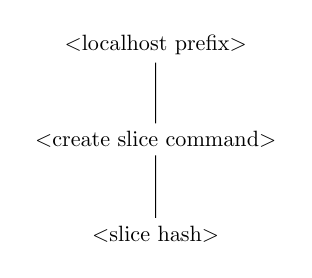
\begin{tikzpicture} [scale=0.8, transform shape]
    %\tikzstyle{every node}=[rectangle,draw]
    \node {$<$localhost prefix$>$}
        child { node {$<$create slice command$>$} 
        		child{ node {$<$slice hash$>$} }
        }
    ;
\end{tikzpicture}
\label{img:repotree}
}
\end{subfigure}
\begin{subfigure} [Discovery Tree]
{
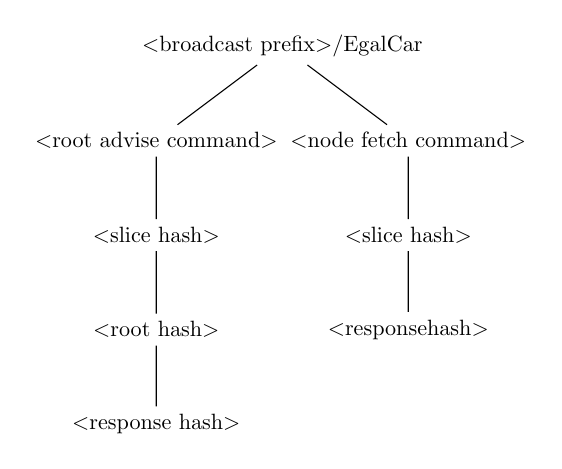
\begin{tikzpicture} [scale=0.8, transform shape]
    \tikzstyle{every node}=[align = center]
    \tikzstyle{level 1} = [sibling distance=40mm]
    \node {$<$broadcast prefix$>$/EgalCar}
        child { node {$<$root advise command$>$} 
        		child { node {$<$slice hash$>$} 
			child { node {$<$root hash$>$} 
				child { node {$<$response hash$>$}} }
		}
        }
        child { node {$<$node fetch command$>$}
        		child { node {$<$slice hash$>$} 
			child { node {$<$responsehash$>$} }
		}
        }
    ;
\end{tikzpicture}
\label{img:discovery}
}
\end{subfigure}
\begin{subfigure} [Game Tree]
{
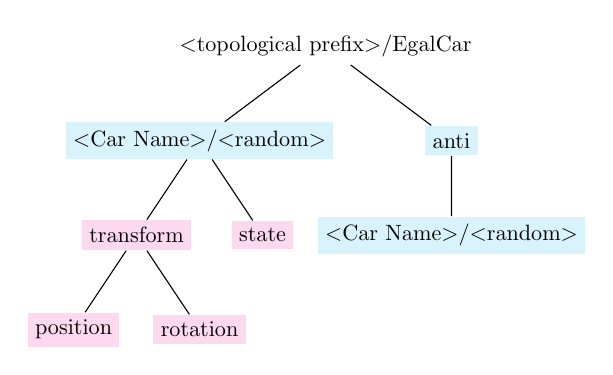
\begin{tikzpicture} [scale=0.8, transform shape]
    \tikzstyle{every node} = [align=center]
    \tikzstyle{asset} = [fill=cyan!15]
    \tikzstyle{state} = [fill=magenta!15]
    \tikzstyle{event} = [fill=orange!15]
    \tikzstyle{level 1} = [sibling distance=40mm]
    \tikzstyle{level 2} = [sibling distance=20mm]
    \node {$<$topological prefix$>$/EgalCar}
        child { node [asset] {$<$Car Name$>$/$<$random$>$} 
		child { node [state] {transform} 
			child{ node [state] {position} }
			child{ node [state] {rotation} }
		}
		child { node [state] {state} }
        }
         child{ node [asset] {anti}
        		child { node [asset] {$<$Car Name$>$/$<$random$>$}}
        }
    ;
\end{tikzpicture}
\label{img:gametree}
}
\end{subfigure}
\caption{The Namespace of Egal Car}
\label{img:namespace}
\end{center}
\end{figure}

The Game Tree (figure~\ref{img:gametree}) collects all asset and state names. For illustration purpose we have colored asset names in blue and state names in pink. The root node is composed the game's environment information (\texttt{<topological prefix>}) and the game's name (\texttt{EgalCar}). Since Egal Car is an application developed by UCLA's team for the NDN project, we decided that our \texttt{<topological prefix>} should be \texttt{/ndn/ucla.edu/apps}. Designers of other NDN games should substitute \texttt{EgalCar} and \texttt{<topological prefix>} with their own values. The left child of the root is an asset name that denotes the existence of a car. This node (and all its child nodes) are dynamically created when a player joins in the game. Since Egal Car is a MOG, there will be more than one \texttt{<Car Name>/<random>} nodes as players discovers about each other (see~\ref{assetsynchronization}). The \texttt{<random>} component, which will be substituted by a random number during run-time, is designed in case there is a name collision in \texttt{<Car Name>}. The right child of the root node is used to mark that a certain player (car) has quitted or disconnected. From our discussion above, the \texttt{anti} node and its child nodes are all assets. The rest nodes are state names, and they are synchronized differently than assets.

In section~\ref{ndnbackground} we mentioned that CCNx Sync brings a lot of conveniences to Egal Car's development. This is indeed the case. Not only does it form a solid basis for asset synchronization, CCNx Sync also provides game discovery and player discovery functionalities intrinsically. Yet for CCNx Sync to work, two other trees (the Repository Tree and the Discovery Tree) are needed in the namespace. The Repository Tree is a collection of names for each game application to communicate with its local repository. The repository is where asset data is stored and synchronized by CCNx Sync. \texttt{<localhost prefix>}, the root node of the Repository Tree, confines the communication scope to localhost. The Discovery Tree is the collection of names used by CCNx Sync. Its root node is similar to that of the Game Tree except that it has a broadcast scope (\texttt{<broadcast prefix>}). Since CCNx Sync is used for ``discoveries'', it is very important for its packets to be broadcasted as potential data publishers may appear anywhere in the network. More details of the Repository Tree and the Discovery Tree will be provided in section~\ref{assetsynchronization}.

%-------------------------------------------------------------------------------------------------------------------------------------%
\subsection{Asset Synchronization}
\label{assetsynchronization}

% CCNx Sync
Asset synchronization is about discoveries. When a peer executes a game program, it needs to discover other peers who are also executing the same program. The other peers also need to promptly discover the newcomer. When a peer quits or becomes disconnected, the other peers in the game need to detect this. In Egal Car, detecting the exit of a player is equivalent to discovering the corresponding \texttt{anti} node.

The discoveries start with the Repository Tree. Upon Egal Car's initialization, it defines a slice in the local repository~\cite{CCNxCS}. A \emph{slice} is a collection of content objects. It is how CCNx Sync manages data to be synchronized. A slice is defined by two names: the \texttt{<broadcast prefix>} and the \texttt{<topological prefix>}. The first name defines CCNx Sync's work scope while the second name is the common name prefix of every name in the slice. The game application informs its local repository about the creation of a slice by writing a slice configuration object to it. The name used in this process is \texttt{<localhost prefix>/<create slice command>/<slice hash>}. \texttt{<localhost prefix>} confines the packet within the same node; \texttt{<create slice command>} claims the command type; \texttt{<slice hash>} is the SHA-256 hash of the slice configuration object and will be used as the name of the slice in the Discovery Tree.

Once the slice is created, CCNx Sync will start sending out \emph{Root Advise} Interests periodically. These Interests are broadcasted on our NDN testbed (as defined by the \texttt{broadcast prefix} during slice creation). Root Advise Interests have names of the form \texttt{.../<root advise command>/<slice hash>/<root hash>}. The function of \texttt{<root advise command>} is similar to that of \texttt{create slice command} in the Repository Tree except that the command has changed. \texttt{<slice hash>} works as the name of the slice. \texttt{<root hash>} is a hash digest of the local slice. By putting \texttt{<slice hash>} into its Root Advise Interest's name, a peer announces its own existence to the network. Other peers running the same program would recognize that peer as a partner because the \texttt{<slice hash>} is the same. By putting \texttt{<root hash>} into its Root Advise Interest's name a peer reports its own data collection to the network. If this \texttt{<root hash>} is the same as everyone else's \texttt{<root hash>}, then all peers are already in sync. If it is not the same, the other peers would respond to the peer's Root Advise Interest with a Data packet named \texttt{.../<root advise command>/<slice hash>/<root hash>/<response hash>} to inform the difference. Upon learning such difference, CCNx Sync will use \emph{Node Fetch} command and normal Interest/Data packets to eliminate such difference.

The next step is to create and announce an avatar that represents the player. In Egal Car this avatar is a red sports car. To announce the existence of the car to the network, a content object named \texttt{<topological prefix>/EgalCar/<Car Name>/<random>} should be written into the network. Using \texttt{<topological prefix>} means that this content object will be part of the slice and thus will be managed by CCNx Sync. \texttt{<Car Name>} and \texttt{<random>} are generated in real time as mentioned in section~\ref{namespace}. The data of this content object is some configuration information of the car (initial position, 3D model's name, player information etc.). As other peers learn about the newcomer through CCNx Sync, they will use the configuration information to instantiate a 3D car model in the given position and mark it with the given player information. When every peer is in sync with all other peers, the car race can begin.

When a player quits, it first writes an \emph{anti-asset} into its own repository. The anti-asset's name will look like \texttt{<topological prefix>/EgalCar/anti/<Car Name>/<random>}, in which the \texttt{<Car Name>} and \texttt{<random>} represents the car that belongs to the quitting player. From CCNx Sync's point of view, synchronizing anti-assets is exactly the same as synchronizing assets. Peers who learn about the anti-asset will destroy the corresponding avatar in their game world. If a player is forced to quit, such as due to network failure, it will not have a chance to write the anti-asset mentioned above. In this case, the anti-asset will be written by other peers who remain connected. 

It should be pointed out that CCNx Sync is an unordered synchronization mechanism. It does not guarantee that assets that are created earlier will be discovered before those that are created later. For example, if Alice and Bob join in Egal Car at about the same time, Alice writes to her repository an object presenting her car, timestamped $T_a$ and Bob writes to his repository an object timestamped $T_b$. $T_a$ and $T_b$ marks the generation time of the two content objects, and they represent the ``official'' time when Alice and Bob join in the game. We assume that $T_a$ is earlier than $T_b$, but this does not mean that the other peers in the network will discovery Alice earlier than they know Bob. For instance, some of them may know Bob first if they have a fast connection to him.

Assets are independent of each other. This explains why we can use unordered synchronization strategy for asset synchronization. Because assets are independent, there is no causal relationship between asset updates, therefore different processing order of asset updates at different peers will not lead to game state inconsistency. Like in our previous example, whether other peers discovery Alice first or they discover Bob first does not matter, as long as both new players are discovered within reasonable time. We could, of course, use one of these (\cite{Chandy, Bryant, Flockstep, Csync, Doptbkt}) ordered game synchronization strategies to keep assets in sync, but that will incur unnecessary delay and degrade game performance. These ordered synchronization algorithms either hold every peer's step to wait for the correct packet to arrive or performs a rollback when a disordering is detected. In our example, if the first approach is taken, every peer is forced to discovery Alice before Bob: after a peer has discovered Alice, it should lock its step until it can be sure that everyone else in the network has also known about Alice; only after that can the peer discover Bob, although Bob's packet might have arrived at the peer a long time ago. On the other hand, if the second approach is taken, peers can discover Bob first, but they will have to rollback to discover Alice, since Alice's packet has an earlier timestamp; after they performed a rollback and discover about Alice, they will have to ``re-discover'' Bob since their earlier knowledge about Bob would have been canceled by the rollback. These ordered synchronization strategies are for updates that are inter-correlated but are not for assets. Using the first approach for asset synchronization will only slow down the global development pace of the game while using the second one will only decrease the game's interactivity and consume a lot of memory (for rollbacks). Therefore neither one is necessary.

Although asset synchronization is unordered, it does need to be reliable. Alice and Bob must be known by all other peers in spite of potential packet losses. NDN is like IP in that it provides a best-effort delivery but does not give reliability. Therefore the synchronization strategy should ensure that all asset updates are effectively delivered. In Egal Car, reliability is guaranteed by CCNx Sync as the synchronization strategy periodically broadcasts Root Advise Interests throughout the timespan of the game. As long as there is a difference between two repositories, their \texttt{<root hash>} would differ, and CCNx Sync would be targeted to eliminate such differences.

%--------------------------------------------------------------------------------------------------------------------------------------%
\subsection{State Synchronization}
\label{statesynchronization}

State is a snapshot of a variable. When all assets become known to the game, all state variables that should be synchronized become clear also. For example, when Alice and Bob are known to the game, then it is clear that both player's child nodes (the pink nodes of the Game Tree in figure~\ref{img:gametree}) are state that should be synchronized. 

State updates and asset updates are different and similar. On the one hand, they are different in that state updates are usually a series of content objects that share a common name while an asset update is usually a single content object with its unique name. For example, asset updates of Alice's car could be either \texttt{.../<AliceCar>/<random>} or \texttt{.../anti/<AliceCar>/<random>}. Both names represents a single content object. State updates of Alice may use this name \texttt{.../<AliceCar>/<random>/transform/position} to refer to Alice's position. Although it is just one constant name, it may actually represent a series of packets generated every hundred milliseconds. Every state update is timestamped, which is how it can be distinguished from its predecessors and successors. On the other hand, state updates and asset updates are similar in that state updates are also independent of each other. Alice and Bob's state will not affect each other: \texttt{.../<AliceCar>/<random>/transform/position} will not cause \texttt{.../<BobCar>/<random>/transform/position} to change. Note that we are not considering the case where Alice and Bob interact with each other. Such interactions will lead to players' state change but they should not be using our state model. We will provide a new model for these interactions in a future paper (see section~\ref{futurework}).

State synchronization should be ordered, but does not need to be reliable. It has to be ordered because continuous state updates share a common name. These state updates should be processed in the order of their generation time (given by their timestamps) in order for peers to understand the chronological relationship among them. This is especially important in NDN where dated state updates are also cached in the web. If state synchronization does not stick to the chronological order, peers' Interests of other peers' state may be satisfied by the same old state generated a long time ago. Another aspect of state synchronization is that it need not to be reliable. Occasional packet misses in a flow of state updates will not hurt. This is because: first, state updates are independent of each other, which means some information missing about Alice's state will not affect a peer's understanding of Bob's state; second, state updates are snapshots rather than change logs, which means that newer state updates will always fully \emph{overwrite} the older state update and little harm will be done if there is a missing state between the two updates. One can compare state synchronization to newspaper delivery. Newspapers should have a printed date and should be delivered in the chronological order in order for newspaper readers to understand the on-going trends of the world. But readers do not have to worry if yesterday's newspaper did not arrive, as today's newspaper will come soon. If the news in yesterday's newspaper is still valid, it will be covered in today's newspaper, too. If it is not valid any more, readers have no reason to care about it.

In Egal Car, state synchronization is achieved setting selectors in Interest packets to retrieve the state in need. 

%============================================================================%
\section{Implementation}
\label{implementation}


%============================================================================%
\section{Future Work}
\label{futurework}


%============================================================================%
\section{Conclusions}
\label{conclusions}


%============================================================================%
\bibliographystyle{plain}
\bibliography{sample}

\end{document}



